\hypertarget{stateful-action}{%
\section{Stateful action}\label{stateful-action}}

Some actions have states. The typical values of states is boolean or
string. However, other types of states are possible if you want.

There's an example \passthrough{\lstinline!menu2\_int16.c!} in the
\passthrough{\lstinline!src/men!} directory. It behaves the same as
\passthrough{\lstinline!menu2.c!}. But it uses gint16 type of states
instead of string type.

Actions which have states are called stateful.

\hypertarget{stateful-action-without-a-parameter}{%
\subsection{Stateful action without a
parameter}\label{stateful-action-without-a-parameter}}

Some menus are called toggle menu. For example, fullscreen menu has a
state which has two values -- fullscreen and non-fullscreen. The value
of the state is changed every time the menu is clicked. An action
corresponds to the fullscreen menu also have a state. Its value is TRUE
or FALSE and it is called boolean value. TRUE corresponds to fullscreen
and FALSE to non-fullscreen.

The following is an example code to implement a fullscreen menu except
the signal handler. The signal handler will be described after the
explanation of this code.

\begin{lstlisting}[language=C]
static void
app_activate (GApplication *app, gpointer user_data) {
  ... ... ...
  GSimpleAction *act_fullscreen = g_simple_action_new_stateful ("fullscreen",
                                  NULL, g_variant_new_boolean (FALSE));
  GMenuItem *menu_item_fullscreen = g_menu_item_new ("Full Screen", "win.fullscreen");
  g_signal_connect (act_fullscreen, "change-state", G_CALLBACK (fullscreen_changed), win);
  ... ... ...
}
\end{lstlisting}

\begin{itemize}
\tightlist
\item
  \passthrough{\lstinline!act\_fullscreen!} is a GSimpleAction instance.
  It is created with
  \passthrough{\lstinline!g\_simple\_action\_new\_stateful!}. The
  function has three arguments. The first argument ``fullscreen'' is the
  name of the action. The second argument is a parameter type.
  \passthrough{\lstinline!NULL!} means the action doesn't have a
  parameter. The third argument is the initial state of the action. It
  is a GVariant value. GVariant will be explained in the next
  subsection. The function
  \passthrough{\lstinline!g\_variant\_new\_boolean (FALSE)!} returns a
  GVariant value which is the boolean value
  \passthrough{\lstinline!FALSE!}.
\item
  \passthrough{\lstinline!menu\_item\_fullscreen!} is a GMenuItem
  instance. There are two arguments. The first argument ``Full Screen''
  is a label of \passthrough{\lstinline!menu\_item\_fullscreen!}. The
  second argument is an action. The action ``win.fullscreen'' has a
  prefix ``win'' and an action name ``fullscreen''. The prefix says that
  the action belongs to the window.
\item
  connects the action \passthrough{\lstinline!act\_fullscreen!} and the
  ``change-state'' signal handler
  \passthrough{\lstinline!fullscreen\_changed!}. If the fullscreen menu
  is clicked, then the corresponding action
  \passthrough{\lstinline!act\_fullscreen!} is activated. But no handler
  is connected to the ``activate'' signal. Then, the default behavior
  for boolean-stated actions with a NULL parameter type like
  \passthrough{\lstinline!act\_fullscreen!} is to toggle them via the
  ``change-state'' signal.
\end{itemize}

The following is the ``change-state'' signal handler.

\begin{lstlisting}[language=C]
static void
fullscreen_changed(GSimpleAction *action, GVariant *value, gpointer win) {
  if (g_variant_get_boolean (value))
    gtk_window_maximize (GTK_WINDOW (win));
  else
    gtk_window_unmaximize (GTK_WINDOW (win));
  g_simple_action_set_state (action, value);
}
\end{lstlisting}

\begin{itemize}
\tightlist
\item
  There are three parameters. The first parameter is the action which
  emits the ``change-state'' signal. The second parameter is the value
  of the new state of the action. The third parameter is a user data
  which is set in \passthrough{\lstinline!g\_signal\_connect!}.
\item
  If the value is boolean type and \passthrough{\lstinline!TRUE!}, then
  it maximizes the window. Otherwise unmaximizes.
\item
  Sets the state of the action with \passthrough{\lstinline!value!}.
  Note: the second argument was the toggled state value, but at this
  stage the state of the action has the original value. So, you need to
  set the state with the new value by
  \passthrough{\lstinline!g\_simple\_action\_set\_state!}.
\end{itemize}

You can use ``activate'' signal instead of ``change-state'' signal, or
both signals. But the way above is the simplest and the best.

\hypertarget{gvariant}{%
\subsubsection{GVariant}\label{gvariant}}

GVarient can contain boolean, string or other type values. For example,
the following program assigns TRUE to \passthrough{\lstinline!value!}
whose type is GVariant.

\begin{lstlisting}[language=C]
GVariant *value = g_variant_new_boolean (TRUE);
\end{lstlisting}

Another example is:

\begin{lstlisting}[language=C]
GVariant *value2 = g_variant_new_string ("Hello");
\end{lstlisting}

\passthrough{\lstinline!value2!} is a GVariant and it has a string type
value ``Hello''. GVariant can contain other types like int16, int32,
int64, double and so on.

If you want to get the original value, use g\_variant\_get series
functions. For example, you can get the boolean value by
g\_variant\_get\_boolean.

\begin{lstlisting}[language=C]
gboolean bool = g_variant_get_boolean (value);
\end{lstlisting}

Because \passthrough{\lstinline!value!} has been created as a boolean
type GVariant and \passthrough{\lstinline!TRUE!} value,
\passthrough{\lstinline!bool!} equals \passthrough{\lstinline!TRUE!}. In
the same way, you can get a string from \passthrough{\lstinline!value2!}

\begin{lstlisting}[language=C]
const char *str = g_variant_get_string (value2, NULL);
\end{lstlisting}

The second parameter is a pointer to gsize type variable (gsize is
defined as unsigned long). If it isn't NULL, then the length of the
string will be set by the function. If it is NULL, nothing happens. The
returned string \passthrough{\lstinline!str!} can't be changed.

\hypertarget{stateful-action-with-a-parameter}{%
\subsection{Stateful action with a
parameter}\label{stateful-action-with-a-parameter}}

Another example of stateful actions is an action corresponds to color
select menus. For example, there are three menus and each menu has red,
green or blue color respectively. They determine the background color of
a certain widget. One action is connected to the three menus. The action
has a state which values are ``red'', ``green'' and ``blue''. The values
are string. Those colors are given to the signal handler as a parameter.

\begin{lstlisting}[language=C]
static void
app_activate (GApplication *app, gpointer user_data) {
  ... ... ...
  GSimpleAction *act_color = g_simple_action_new_stateful ("color",
                     g_variant_type_new("s"), g_variant_new_string ("red"));
  GMenuItem *menu_item_red = g_menu_item_new ("Red", "win.color::red");
  GMenuItem *menu_item_green = g_menu_item_new ("Green", "win.color::green");
  GMenuItem *menu_item_blue = g_menu_item_new ("Blue", "win.color::blue");
  g_signal_connect (act_color, "activate", G_CALLBACK (color_activated), win);
  ... ... ...
}
\end{lstlisting}

\begin{itemize}
\tightlist
\item
  \passthrough{\lstinline!act\_color!} is a GSimpleAction instance. It
  is created with
  \passthrough{\lstinline!g\_simple\_action\_new\_stateful!}. The
  function has three arguments. The first argument ``color'' is the name
  of the action. The second argument is a parameter type which is
  GVariantType. \passthrough{\lstinline!g\_variant\_type\_new("s")!}
  creates GVariantType which is a string type
  (\passthrough{\lstinline!G\_VARIANT\_TYPE\_STRING!}). The third
  argument is the initial state of the action. It is a GVariant.
  GVariantType will be explained in the next subsection. The function
  \passthrough{\lstinline!g\_variant\_new\_string ("red")!} returns a
  GVariant value which has the string value ``red''.
\item
  \passthrough{\lstinline!menu\_item\_red!} is a GMenuItem instance.
  There are two arguments. The first argument ``Red'' is the label of
  \passthrough{\lstinline!menu\_item\_red!}. The second argument is a
  detailed action. Its prefix is ``win'', action name is ``color'' and
  target is ``red''. Target is sent to the action as a parameter. The
  same goes for \passthrough{\lstinline!menu\_item\_green!} and
  \passthrough{\lstinline!menu\_item\_blue!}.
\item
  connects the action \passthrough{\lstinline!act\_color!} and the
  ``activate'' signal handler
  \passthrough{\lstinline!color\_activated!}. If one of the three menus
  is clicked, then the action \passthrough{\lstinline!act\_color!} is
  activated with the target (parameter) which is given by the menu. No
  handler is connected to ``change-state'' signal. Then the default
  behavior is to call
  \passthrough{\lstinline!g\_simple\_action\_set\_state()!} to set the
  state to the requested value.
\end{itemize}

The following is the ``activate'' signal handler.

\begin{lstlisting}[language=C]
static void
color_activated(GSimpleAction *action, GVariant *parameter, gpointer win) {
  char *color = g_strdup_printf ("label#lb {background-color: %s;}",
                                   g_variant_get_string (parameter, NULL));
  gtk_css_provider_load_from_data (provider, color, -1);
  g_free (color);
  g_action_change_state (G_ACTION (action), parameter);
}
\end{lstlisting}

\begin{itemize}
\tightlist
\item
  There are three parameters. The first parameter is the action which
  emits the ``activate'' signal. The second parameter is the parameter
  given to the action. It is a color specified by the menu. The third
  parameter is a user data which is set in
  \passthrough{\lstinline!g\_signal\_connect!}.
\item
  \passthrough{\lstinline!color!} is a CSS string created by
  \passthrough{\lstinline!g\_strdup\_printf!}. The parameter of
  \passthrough{\lstinline!g\_strdup\_printf!} is the same as printf C
  standard function. \passthrough{\lstinline!g\_variant\_get\_string!}
  gets the string contained in \passthrough{\lstinline!parameter!}. You
  mustn't change or free the string.
\item
  Sets the color of the css provider.
\item
  Frees the string \passthrough{\lstinline!color!}.
\item
  Changes the state by
  \passthrough{\lstinline!g\_action\_change\_state!}. The function just
  sets the state of the action to the parameter by
  \passthrough{\lstinline!g\_simple\_action\_set\_state!}. Therefore,
  you can use \passthrough{\lstinline!g\_simple\_action\_set\_state!}
  instead of \passthrough{\lstinline!g\_action\_change\_state!}.
\end{itemize}

Note: If you have set a ``change-state'' signal handler,
\passthrough{\lstinline!g\_action\_change\_state!} will emit
``change-state'' signal instead of calling
\passthrough{\lstinline!g\_simple\_action\_set\_state!}.

\hypertarget{gvarianttype}{%
\subsubsection{GVariantType}\label{gvarianttype}}

GVariantType gives a type of GVariant. GVariant can contain many kinds
of types. And the type often needs to be recognized at runtime.
GVariantType provides such functionality.

GVariantType is created with a string which expresses a type.

\begin{itemize}
\tightlist
\item
  ``b'' means boolean type.
\item
  ``s'' means string type.
\end{itemize}

The following program is a simple example. It finally outputs the string
``s''.

\begin{lstlisting}[language=C, numbers=left]
#include <glib.h>

int
main (int argc, char **argv) {
  GVariantType *vtype = g_variant_type_new ("s");
  const char *type_string = g_variant_type_peek_string (vtype);
  g_print ("%s\n",type_string);
}
\end{lstlisting}

\begin{itemize}
\tightlist
\item
  \passthrough{\lstinline!g\_variant\_type\_new!} creates GVariantType.
  It uses a type string ``s'' which means string.
\item
  \passthrough{\lstinline!g\_variant\_type\_peek\_string!} takes a peek
  at \passthrough{\lstinline!vtype!}. It is the string ``s'' given to
  \passthrough{\lstinline!vtype!} when it was created.
\item
  prints the string to the terminal.
\end{itemize}

\hypertarget{example-code}{%
\subsection{Example code}\label{example-code}}

The following code includes stateful actions above. This program has
menus like this:

\begin{figure}
\centering
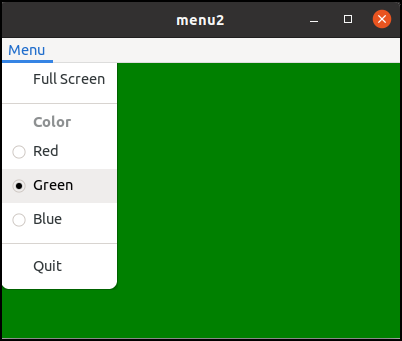
\includegraphics[width=6.03cm,height=5.115cm]{../image/menu2.png}
\caption{menu2}
\end{figure}

\begin{itemize}
\tightlist
\item
  Fullscreen menu toggles the size of the window between maximum and
  non-maximum. If the window is maximum size, which is called full
  screen, then a check mark is put before ``fullscreen'' label.
\item
  Red, green and blue menu determines the back ground color of the
  label, which is the child widget of the window. The menus have radio
  buttons on the left of the menus. And the radio button of the selected
  menu turns on.
\item
  Quit menu quits the application.
\end{itemize}

The code is as follows.

\begin{lstlisting}[language=C, numbers=left]
#include <gtk/gtk.h>

static GtkCssProvider *provider;

static void
fullscreen_changed(GSimpleAction *action, GVariant *value, gpointer win) {
  if (g_variant_get_boolean (value))
    gtk_window_maximize (GTK_WINDOW (win));
  else
    gtk_window_unmaximize (GTK_WINDOW (win));
  g_simple_action_set_state (action, value);
}

static void
color_activated(GSimpleAction *action, GVariant *parameter, gpointer win) {
  char *color = g_strdup_printf ("label#lb {background-color: %s;}", g_variant_get_string (parameter, NULL));
  gtk_css_provider_load_from_data (provider, color, -1);
  g_free (color);
  g_action_change_state (G_ACTION (action), parameter);
}

static void
quit_activated(GSimpleAction *action, GVariant *parameter, gpointer app)
{
  g_application_quit (G_APPLICATION(app));
}

static void
app_activate (GApplication *app, gpointer user_data) {
  GtkWidget *win = gtk_application_window_new (GTK_APPLICATION (app));
  gtk_window_set_title (GTK_WINDOW (win), "menu2");
  gtk_window_set_default_size (GTK_WINDOW (win), 400, 300);

  GtkWidget *lb = gtk_label_new (NULL);
  gtk_widget_set_name (lb, "lb"); /* the name is used by CSS Selector */
  gtk_window_set_child (GTK_WINDOW (win), lb);

  GSimpleAction *act_fullscreen
    = g_simple_action_new_stateful ("fullscreen", NULL, g_variant_new_boolean (FALSE));
  GSimpleAction *act_color
    = g_simple_action_new_stateful ("color", g_variant_type_new("s"), g_variant_new_string ("red"));
  GSimpleAction *act_quit
    = g_simple_action_new ("quit", NULL);

  GMenu *menubar = g_menu_new ();
  GMenu *menu = g_menu_new ();
  GMenu *section1 = g_menu_new ();
  GMenu *section2 = g_menu_new ();
  GMenu *section3 = g_menu_new ();
  GMenuItem *menu_item_fullscreen = g_menu_item_new ("Full Screen", "win.fullscreen");
  GMenuItem *menu_item_red = g_menu_item_new ("Red", "win.color::red");
  GMenuItem *menu_item_green = g_menu_item_new ("Green", "win.color::green");
  GMenuItem *menu_item_blue = g_menu_item_new ("Blue", "win.color::blue");
  GMenuItem *menu_item_quit = g_menu_item_new ("Quit", "app.quit");

  g_signal_connect (act_fullscreen, "change-state", G_CALLBACK (fullscreen_changed), win);
  g_signal_connect (act_color, "activate", G_CALLBACK (color_activated), win);
  g_signal_connect (act_quit, "activate", G_CALLBACK (quit_activated), app);
  g_action_map_add_action (G_ACTION_MAP (win), G_ACTION (act_fullscreen));
  g_action_map_add_action (G_ACTION_MAP (win), G_ACTION (act_color));
  g_action_map_add_action (G_ACTION_MAP (app), G_ACTION (act_quit));

  g_menu_append_item (section1, menu_item_fullscreen);
  g_menu_append_item (section2, menu_item_red);
  g_menu_append_item (section2, menu_item_green);
  g_menu_append_item (section2, menu_item_blue);
  g_menu_append_item (section3, menu_item_quit);
  g_object_unref (menu_item_red);
  g_object_unref (menu_item_green);
  g_object_unref (menu_item_blue);
  g_object_unref (menu_item_fullscreen);
  g_object_unref (menu_item_quit);

  g_menu_append_section (menu, NULL, G_MENU_MODEL (section1));
  g_menu_append_section (menu, "Color", G_MENU_MODEL (section2));
  g_menu_append_section (menu, NULL, G_MENU_MODEL (section3));
  g_menu_append_submenu (menubar, "Menu", G_MENU_MODEL (menu));

  gtk_application_set_menubar (GTK_APPLICATION (app), G_MENU_MODEL (menubar));
  gtk_application_window_set_show_menubar (GTK_APPLICATION_WINDOW (win), TRUE);

/*  GtkCssProvider *provider = gtk_css_provider_new ();*/
  provider = gtk_css_provider_new ();
  GdkDisplay *display = gtk_widget_get_display (GTK_WIDGET (win));
  gtk_css_provider_load_from_data (provider, "label#lb {background-color: red;}", -1);
  gtk_style_context_add_provider_for_display (display, GTK_STYLE_PROVIDER (provider),
                                              GTK_STYLE_PROVIDER_PRIORITY_USER);

/*  gtk_widget_show (win);*/
  gtk_window_present (GTK_WINDOW (win));
}

#define APPLICATION_ID "com.github.ToshioCP.menu2"

int
main (int argc, char **argv) {
  GtkApplication *app;
  int stat;

  app = gtk_application_new (APPLICATION_ID, G_APPLICATION_FLAGS_NONE);
  g_signal_connect (app, "activate", G_CALLBACK (app_activate), NULL);

  stat =g_application_run (G_APPLICATION (app), argc, argv);
  g_object_unref (app);
  return stat;
}
\end{lstlisting}

\begin{itemize}
\tightlist
\item
  5-26: Signal handlers. They have already been explained.
\item
  30-36: \passthrough{\lstinline!win!} and \passthrough{\lstinline!lb!}
  are GtkApplicationWindow and GtkLabel respectively.
  \passthrough{\lstinline!win!} has a title ``menu2'' and its default
  size is 400x300. \passthrough{\lstinline!lb!} is named as ``lb''. The
  name is used in CSS. \passthrough{\lstinline!lb!} is set to
  \passthrough{\lstinline!win!} as a child.
\item
  38-43: Three actions are defined. They are:

  \begin{itemize}
  \tightlist
  \item
    stateful and has no parameter. It has a toggle state.
  \item
    stateful and has a parameter. Parameter is a string type.
  \item
    stateless and has no parameter.
  \end{itemize}
\item
  45-54: Creates GMenu and GMenuItem. There are three sections.
\item
  56-61: Signals are connected to handlers. And actions are added to
  GActionMap. Because \passthrough{\lstinline!act\_fullscreen!} and
  \passthrough{\lstinline!act\_color!} have ``win'' prefix and belong to
  GtkApplicationWindow, they are added to \passthrough{\lstinline!win!}.
  GtkApplicationWindow implements GActionModel interface like
  GtkApplication. \passthrough{\lstinline!act\_quit!} has ``app'' prefix
  and belongs to GtkApplication. It is added to
  \passthrough{\lstinline!app!}.
\item
  63-77: Connects and builds the menus. Useless GMenuItem are freed.
\item
  79-80: GMenuModel \passthrough{\lstinline!menubar!} is inserted to
  \passthrough{\lstinline!app!}. Sets show menubar property of
  \passthrough{\lstinline!win!} to \passthrough{\lstinline!TRUE!}. Note:
  \passthrough{\lstinline!gtk\_application\_window\_set\_show\_menubar!}
  creates GtkPopoverMenubar from GMenuModel. This is a different point
  between Gtk3 and Gtk4. And you can use GtkPopoverMenubar directly and
  set it as a descendant widget of the window. You may use GtkBox as a
  child widget of the window and insert GtkPopoverMenubar as the first
  child of the box.
\item
  82-87: Sets CSS. \passthrough{\lstinline!provider!} is GtkCssProvider
  which is defined in line three as a static variable. Its CSS data is:
  \passthrough{\lstinline!label\#lb \{background-color: red;\}!}.
  ``label\#lb'' is called selector. ``label'' is the node of GtkLabel.
  ``\#'' precedes an ID which is an identifiable name of the widget.
  ``lb'' is the name of GtkLabel \passthrough{\lstinline!lb!}. (See line
  35). The style is surrounded by open and close braces. The style is
  applied to GtkLabel which has a name ``lb''. Other GtkLabel have no
  effect from this. The provider is added to GdkDisplay.
\item
  90: Shows the window.
\end{itemize}
